\documentclass{article}

\usepackage{graphicx}
\usepackage{rotating}
\usepackage{amsmath}
\usepackage{fancyhdr}
\usepackage{listings}
\usepackage{xcolor}
\usepackage{color}
\usepackage{textcomp}
\usepackage{float}
\usepackage{multirow}
\usepackage[sorting=none]{biblatex}
\usepackage[margin=1in]{geometry}
\usepackage[font={small,it}]{caption}
\usepackage{placeins}
\usepackage{xepersian}

%\DeclareMathOperator*{\btie}{\bowtie}
\addbibresource{bibliography.bib}
\settextfont[Scale=1.2]{B-NAZANIN.TTF}
\setlatintextfont[Scale=1]{Times New Roman}
\renewcommand{\baselinestretch}{1.5}
\pagestyle{fancy}
\fancyhf{}
\rhead{تکلیف سوم درس مبانی بینایی کامپیوتر}
\lhead{\thepage}
\rfoot{علیرضا ابره فروش}
\lfoot{9816603}
\renewcommand{\headrulewidth}{1pt}
\renewcommand{\footrulewidth}{1pt}
%%%%%%%%%%
\lstset
{
    language=[latex]tex,
    basicstyle=\ttfamily,
    commentstyle=\color{black},
    columns=fullflexible,
    keepspaces=true,
    upquote=true,
    showstringspaces=false,
    morestring=[s]\\\%,
    stringstyle=\color{black},
}
%%%%%%%%%%
%beginMatlab
\definecolor{mygreen}{RGB}{28,172,0} % color values Red, Green, Blue
\definecolor{mylilas}{RGB}{170,55,241}
%endMatlab
\begin{document}
%beginMatlab
\lstset{language=Matlab,%
    %basicstyle=\color{red},
    breaklines=true,%
    morekeywords={matlab2tikz},
    keywordstyle=\color{blue},%
    morekeywords=[2]{1}, keywordstyle=[2]{\color{black}},
    identifierstyle=\color{black},%
    stringstyle=\color{mylilas},
    commentstyle=\color{mygreen},%
    showstringspaces=false,%without this there will be a symbol in the places where there is a space
    numbers=left,%
    numberstyle={\tiny \color{black}},% size of the numbers
    numbersep=9pt, % this defines how far the numbers are from the text
    emph=[1]{for,end,break},emphstyle=[1]\color{red}, %some words to emphasise
    %emph=[2]{word1,word2}, emphstyle=[2]{style},    
}
%endMatlab
\begin{titlepage}
\begin{center}

\includegraphics[width=0.4\textwidth]{figures/IUT Logo.png}\\
        
\LARGE
\textbf{دانشگاه صنعتی اصفهان}\\
\textbf{دانشکده مهندسی برق و کامپیوتر}\\
        
\vfill
        
\huge
\textbf{عنوان: تکلیف چهارم درس ریزپردازنده}\\
        
\vfill
        
\LARGE
\textbf{نام و نام خانوادگی: علیرضا ابره فروش}\\
\textbf{شماره دانشجویی: 9816603}\\
\textbf{نیم\,سال تحصیلی: پاییز 1400}\\
\textbf{مدرّس: دکتر عارف کریمی افشار}\\
\end{center}
\end{titlepage}


%\tableofcontents
\newpage


\section{}%1
\begin{figure}[H]
    \centering
    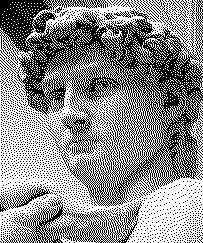
\includegraphics[width=0.25\textwidth]{figures/3c1.jpg}
    \caption
	{
خروجی الگوریتم \lr{Floyd-Steinberg}
	}
    \label{fig:fig1}
\end{figure}
\begin{figure}[H]
    \centering
    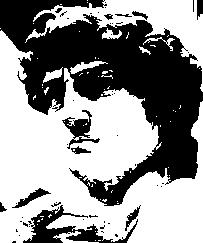
\includegraphics[width=0.25\textwidth]{figures/3c2.jpg}
    \caption
	{
خروجی الگوریتم حریصانه
	}
    \label{fig:fig1}
\end{figure}
\section{}%2
\section{}%3
\section{}%4
\subsection{\lr{Algorithm}}
برای هر پیکسل دارای نویز فلفل نمکی (سطح روشنایی 0 و 255) یک کرنل 3 در 3 نظر می‌گیریم و آن را با میانگین سطح روشنایی پیکسل‌های همسایه‌اش در کرنل 3 در 3 که دارای نویز نیستند (در صورت وجود) مقداردهی می‌کنیم.سطح روشنایی سایر پیکسل‌ها (که یا همه‌ی همسایه‌هاشان نویز هستند یا خودشان فاقد نویز) را بدون تغییر می‌گذاریم. با فرض اینکه تصویر اصلی فاقد سطح روشنایی 0 یا 255 باشد (یا به تعداد کم) الگوریتم را تا جایی که هیچ پیکسل با سطح روشنایی 0 یا 255 باقی نماند تکرار می‌کنیم. این کار در تصاویر با نویز بالا که در آن بسیاری از پیکسل‌ها در همسایگی‌های 3 در 3ی خود همسایه‌ی غیر نویز ندارند می‌تواند تا حدی کیفیت تصاویر را ارتقا دهد. توجه شود که در صورتی که تصویر اصلی تعداد زیادی پیکسل 0 یا 255 داشته باشد آنگاه این الگوریتم ناکارآمد است. همچنین با توجه به اینکه ممکن است الگوریتم به تعداد زیادی اجرا شود (با توجه به درصد نویز و میزان پراکندگی آن) در کاربردهایی که زمان اهمیت دارد می‌تواند نا کارآمد باشد.
\subsection{\lr{Function}}
\begin{latin}
\lstinputlisting{sources/removeNoise.m}
\end{latin}

\subsection{\lr{Driver Code}}
\begin{latin}
\lstinputlisting{sources/p4.m}
\end{latin}

\subsection{\lr{Results}}
%table
% Please add the following required packages to your document preamble:
% \usepackage{multirow}
\begin{table}[H]
\begin{tabular}{|cccccccc|c|}
\hline
\multicolumn{8}{|c|}{\textbf{مقدار \lr{PSNR}}}                                                                                                                                                                                                                                                                                                    & \multirow{3}{*}{\textbf{مقدار نویز}} \\ \cline{1-8}
\multicolumn{2}{|c|}{\textbf{\lr{House}}}                                                & \multicolumn{2}{c|}{\textbf{\lr{Peppers}}}                                              & \multicolumn{2}{c|}{\textbf{\lr{Boat}}}                                                 & \multicolumn{2}{c|}{\textbf{\lr{Bridge}}}                          &                                      \\ \cline{1-8}
\multicolumn{1}{|c|}{\textbf{روش شما}}      & \multicolumn{1}{c|}{\textbf{\lr{Median}}}  & \multicolumn{1}{c|}{\textbf{روش شما}}      & \multicolumn{1}{c|}{\textbf{\lr{Median}}}  & \multicolumn{1}{c|}{\textbf{روش شما}}      & \multicolumn{1}{c|}{\textbf{\lr{Median}}}  & \multicolumn{1}{c|}{\textbf{روش شما}}      & \textbf{\lr{Median}}  &                                      \\ \hline
\multicolumn{1}{|c|}{\lr{41.3155}}          & \multicolumn{1}{c|}{\lr{31.6136}}          & \multicolumn{1}{c|}{\lr{40.1790}}          & \multicolumn{1}{c|}{\lr{32.9933}}          & \multicolumn{1}{c|}{\lr{38.3188}}          & \multicolumn{1}{c|}{\lr{29.5452}}          & \multicolumn{1}{c|}{\lr{35.4940}}          & \lr{26.4491}          & \textbf{10\%}                        \\ \hline
\multicolumn{1}{|c|}{\lr{37.8877}}          & \multicolumn{1}{c|}{\lr{27.1770}}          & \multicolumn{1}{c|}{\lr{37.1491}}          & \multicolumn{1}{c|}{\lr{28.5689}}          & \multicolumn{1}{c|}{\lr{35.1236}}          & \multicolumn{1}{c|}{\lr{26.8926}}          & \multicolumn{1}{c|}{\lr{32.3510}}          & \lr{24.7149}          & \textbf{20\%}                        \\ \hline
\multicolumn{1}{|c|}{\lr{35.5075}}          & \multicolumn{1}{c|}{\lr{22.1984}}          & \multicolumn{1}{c|}{\lr{34.8541}}          & \multicolumn{1}{c|}{\lr{23.3094}}          & \multicolumn{1}{c|}{\lr{32.9896}}          & \multicolumn{1}{c|}{\lr{22.8737}}          & \multicolumn{1}{c|}{\lr{30.3924}}          & \lr{21.6692}          & \textbf{30\%}                        \\ \hline
\multicolumn{1}{|c|}{\lr{33.9004}}          & \multicolumn{1}{c|}{\lr{18.3001}}          & \multicolumn{1}{c|}{\lr{33.2457}}          & \multicolumn{1}{c|}{\lr{18.7179}}          & \multicolumn{1}{c|}{\lr{31.4095}}          & \multicolumn{1}{c|}{\lr{18.6787}}          & \multicolumn{1}{c|}{\lr{28.7389}}          & \lr{17.8907}          & \textbf{40\%}                        \\ \hline
\multicolumn{1}{|c|}{\lr{31.9559}}          & \multicolumn{1}{c|}{\lr{15.1437}}          & \multicolumn{1}{c|}{\lr{31.7296}}          & \multicolumn{1}{c|}{\lr{15.2770}}          & \multicolumn{1}{c|}{\lr{29.9644}}          & \multicolumn{1}{c|}{\lr{15.2068}}          & \multicolumn{1}{c|}{\lr{27.3220}}          & \lr{14.6175}          & \textbf{50\%}                        \\ \hline
\multicolumn{1}{|c|}{\lr{29.7612}}          & \multicolumn{1}{c|}{\lr{12.3490}}          & \multicolumn{1}{c|}{\lr{30.0131}}          & \multicolumn{1}{c|}{\lr{12.1137}}          & \multicolumn{1}{c|}{\lr{28.4694}}          & \multicolumn{1}{c|}{\lr{12.3400}}          & \multicolumn{1}{c|}{\lr{25.8672}}          & \lr{11.9099}          & \textbf{60\%}                        \\ \hline
\multicolumn{1}{|c|}{\lr{28.0489}}          & \multicolumn{1}{c|}{\lr{9.8242}}           & \multicolumn{1}{c|}{\lr{28.2534}}          & \multicolumn{1}{c|}{\lr{9.8964}}           & \multicolumn{1}{c|}{\lr{26.6358}}          & \multicolumn{1}{c|}{\lr{9.9814}}           & \multicolumn{1}{c|}{\lr{24.3418}}          & \lr{9.6961}           & \textbf{70\%}                        \\ \hline
\multicolumn{1}{|c|}{\lr{25.7710}}          & \multicolumn{1}{c|}{\lr{8.0907}}           & \multicolumn{1}{c|}{\lr{25.8364}}          & \multicolumn{1}{c|}{\lr{7.9913}}           & \multicolumn{1}{c|}{\lr{24.7047}}          & \multicolumn{1}{c|}{\lr{8.1553}}           & \multicolumn{1}{c|}{\lr{22.5651}}          & \lr{7.8965}           & \textbf{80\%}                        \\ \hline
\multicolumn{1}{|c|}{\lr{22.4929}}          & \multicolumn{1}{c|}{\lr{6.6512}}           & \multicolumn{1}{c|}{\lr{22.4505}}          & \multicolumn{1}{c|}{\lr{6.4746}}           & \multicolumn{1}{c|}{\lr{21.7863}}          & \multicolumn{1}{c|}{\lr{6.6309}}           & \multicolumn{1}{c|}{\lr{20.1695}}          & \lr{6.4464}           & \textbf{90\%}                        \\ \hline
\multicolumn{1}{|c|}{\textbf{\lr{31.8490}}} & \multicolumn{1}{c|}{\textbf{\lr{16.8164}}} & \multicolumn{1}{c|}{\textbf{\lr{31.5234}}} & \multicolumn{1}{c|}{\textbf{\lr{17.2603}}} & \multicolumn{1}{c|}{\textbf{\lr{29.9336}}} & \multicolumn{1}{c|}{\textbf{\lr{16.7005}}} & \multicolumn{1}{c|}{\textbf{\lr{27.4713}}} & \textbf{\lr{15.6989}} & \textbf{میانگین}                     \\ \hline
\end{tabular}
\end{table}
%table





%%%%%%%%%%%%%%%%%%%%%%%%%%%%%%%%%%%


%\begin{latin}
%\lstinputlisting{sources/p1.m}
%\end{latin}



%%%%%%%%%%%%%%%%%%%%%%%%%%%%%%%%%%%
%%%%%%%%%%%%%%%%%%%%%%%%%%%%%%%%%%%
%%%%%%%%%%%%%%%%%%%%%%%%%%%%%%%%%%%

%------------------------------------------------------------------------------------------


\section*{منابع}
\renewcommand{\section}[2]{}%
\begin{thebibliography}{99} % assumes less than 100 references
%چنانچه مرجع فارسی نیز داشته باشید باید دستور فوق را فعال کنید و مراجع فارسی خود را بعد از این دستور وارد کنید


\begin{LTRitems}

\resetlatinfont

\bibitem{b1}
\end{LTRitems}

\end{thebibliography}


\end{document}
